\chapter{\introductionname}
\label{chap:introduction}

\subsection{ICOS}

Il livello dei gas serra nell'atmosfera cresce costantemente, riscaldando il nostro pianeta. Osservare 
i livelli di emissioni di questi gas è essenziale per contrastare il cambiamento climatico e mitigarne le 
conseguenze. \\

Il sistema ICOS (Integrated Carbon Observation System) è un sistema europeo creato nel 2007 come parte della ricerca 
ambientale europea, con l'obiettivo di sviluppare una rete di osservazione del carbonio in Europa
in grado di monitorare le emissioni e gli assorbimenti di CO2, nonché di altri gas serra,
in ambienti terrestri e marini. \\

ICOS si basa su una vasta rete di stazioni di misura che coprono tutta l'Europa e che forniscono 
dati di alta qualità sul bilancio del carbonio. Queste stazioni di misura sono distribuite in 
tutta Europa in modo da rappresentare una vasta gamma di ambienti, come foreste, prati, paludi,
zone umide, fiumi e oceani. Le stazioni utilizzano tecnologie avanzate per misurare il flusso
di gas serra in queste diverse ambientazioni, come ad esempio la tecnologia di campionamento 
automatico per l'acqua e l'aria, la misurazione del radon e la tecnologia satellitare.\\

ICOS raccoglie questi dati ambientali per valutare l'impatto del cambiamento climatico
sul ciclo del carbonio e per sviluppare strategie per mitigare l'impatto delle attività
umane sul clima. La raccolta e l'analisi dei dati di ICOS sono supportati da tecnologie 
avanzate del web semantico, che consentono la gestione, l'analisi e la condivisione dei dati 
ambientali in modo efficace ed efficiente. \\

ICOS è stato sviluppato in collaborazione con altri sistemi di osservazione globale del carbonio,
come il Global Carbon Project e il Copernicus Climate Change Service.
Il sistema ICOS è stato riconosciuto come una risorsa essenziale per la comprensione
del bilancio del carbonio in Europa e nel mondo, e il suo contributo è stato riconosciuto
dalla comunità scientifica e dalle organizzazioni internazionali, come il Panel Intergovernativo
sui Cambiamenti Climatici (IPCC) e l'Organizzazione per la Cooperazione e lo Sviluppo Economico (OCSE). \\

\subsection{Structure}

Il progetto ICOS è suddiviso in tre domini: \textbf{Atmosfera} - \textbf{Ecosistema} - \textbf{Oceano}. \\

L'unità fondamentale di ICOS sono le \textbf{ICOS Station Networks} che sono coordinate e gestite dall'
\textbf{ICOS National Networks}. \\

Le \textbf{MSA} (\textit{Monitoring Station Assembly}) sono assemble che studiano e discutono come migliorare
l'osservazione degli ambienti nelle stazioni, cercando di portare novità sia dal punto di vista tecnico che scientifico.
È presente un MSA per ognuno dei tre domini. \\

Le \textbf{Central Facilities} sono entità che coordinano il supporto alle stazione. Ogni dominio ha la sua Central Facility. \\

\begin{figure}[H]
    \caption{ICOS structure}
    \centering
    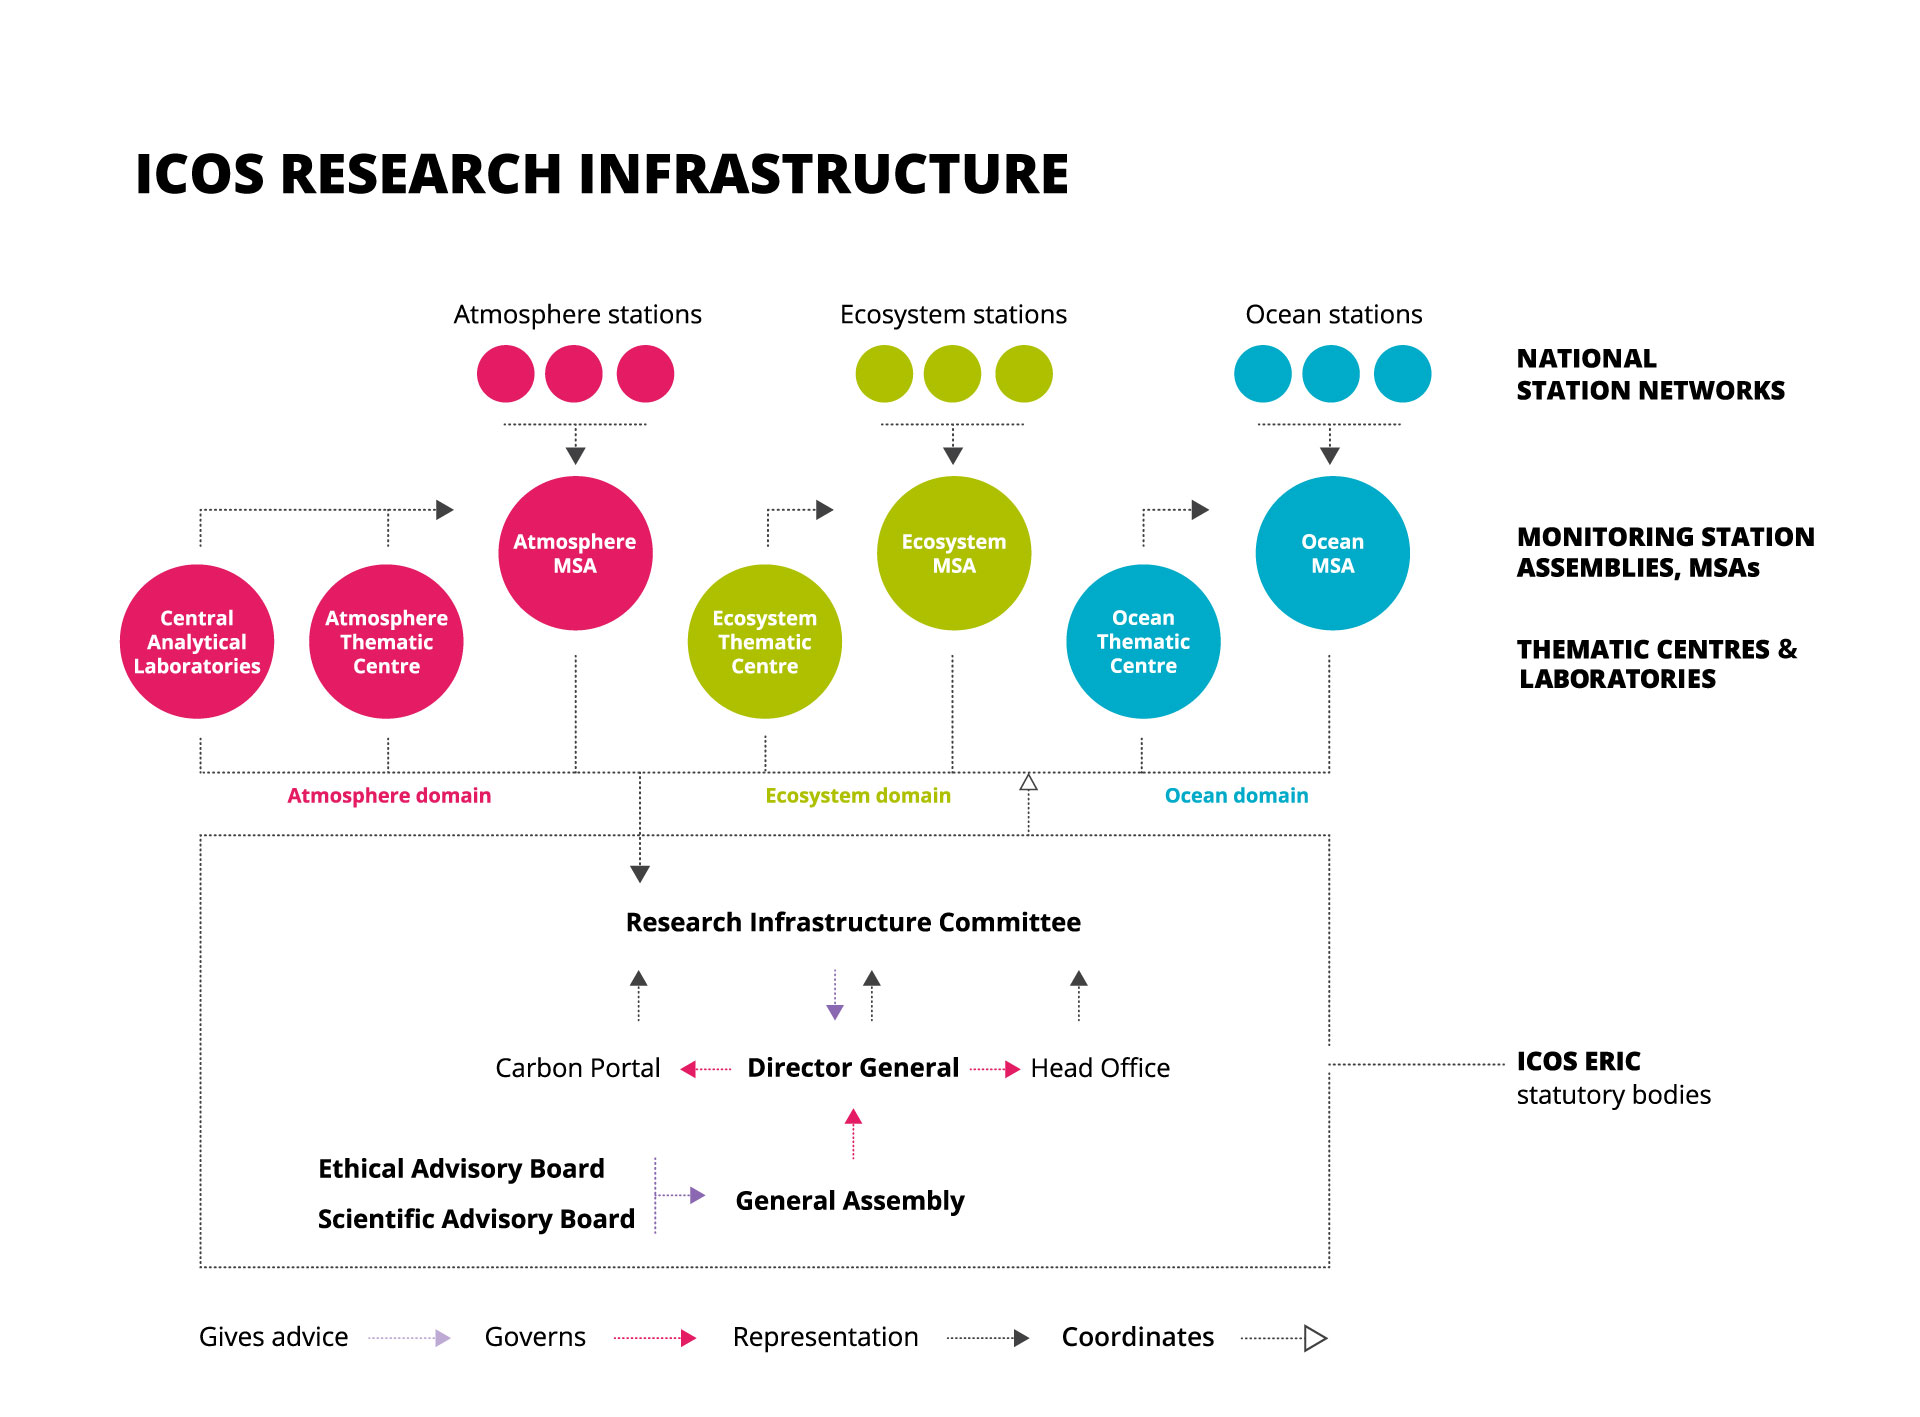
\includegraphics[width=\textwidth]{figures/icos-structure.png}
\end{figure}